\documentclass[11pt,letterpaper]{article}
\usepackage[utf8]{inputenc}
\usepackage[left=1in,right=1in,top=1in,bottom=1in]{geometry}
\usepackage{amsfonts,amsmath}
\usepackage{graphicx,float}
% -----------------------------------
\usepackage{hyperref}
\hypersetup{%
  colorlinks=true,
  linkcolor=blue,
  citecolor=blue,
  urlcolor=blue,
  linkbordercolor={0 0 1}
}
% -----------------------------------
\usepackage[style=authoryear-icomp,backend=biber]{biblatex}
\addbibresource{citation.bib}
% -----------------------------------
\title{Using penalty immersed boundary method to simulate lee wave past topography}
\author{Ryan Sh\`iji\'e D\`u}
\date{\today}
% -----------------------------------
% \setlength{\parindent}{0.0in}
\setlength{\parskip}{0.1in}
% -----------------------------------
\newcommand{\de}{\mathrm{d}}
\newcommand{\DD}{\mathrm{D}}
\newcommand{\pe}{\partial}
\newcommand{\mcal}{\mathcal}
%\newcommand{\pdx}{\left|\frac{\partial}{\partial_x}\right|}

\newcommand{\dsp}{\displaystyle}

\newcommand{\norm}[1]{\left\Vert #1 \right\Vert}
%\newcommand{\mean}[1]{\left\langle #1 \right\rangle}
\newcommand{\mean}[1]{\overline{#1}}
\newcommand{\inner}[2]{\left\langle #1,#2\right\rangle}

\newcommand{\ve}[1]{\boldsymbol{#1}}

\newcommand{\thus}{\Rightarrow \quad }
\newcommand{\fff}{\iff\quad}
\newcommand{\qdt}[1]{\quad \mbox{#1} \quad}

\renewcommand{\Re}{\mathrm{Re}}
\renewcommand{\Im}{\mathrm{Im}}
\newcommand{\E}{\mathbb{E}}
\newcommand{\lap} {\nabla^2}
\renewcommand{\div}{\nabla\cdot}

\newcommand{\csch}{\text{csch}}
\newcommand{\sech}{\text{sech}}


\newcommand{\hot}{\text{h.o.t.}}
\newcommand{\Fr}{\text{Fr}}

\newcommand{\ssp}{\left.\qquad\right.}

\newcommand{\var}{\text{var}}
\newcommand{\cov}{\text{cov}}

\DeclareMathOperator{\supp}{supp}
\begin{document}
% -----------------------------------
\maketitle

\section{Introduction}
Inertial-gravity waves are ubiquitous in the earth's ocean and atmosphere. They are also speculated to exist in extraterrestrial planets. In addition to giving clouds interesting wave patterns (see figures in \cite{YigitMedvedev_19}), their propagation and breaking leads to turbulence which contribute to the mixing of tracers and momentum in the ocean and atmosphere. 

One particular example of inertial-gravity waves is lee waves. When a stratified fluid flow past a topographic feature (e.g.: the jet stream over the Rocky or the Antarctic Circumpolar Current over the Drake passage), it is perturbed by the topography into wave motion. In this note, we will study 2D ($x-z$) gravity waves of stratified fluids over simple topography features. The inertial part represents the effects of the rotation of the earth, which we will leave out for our study. 

We use the penalty immersed boundary method (pIBM) to simulate the topography boundary as well as the fluid's density variation \parencite{KimPeskin_16}. This allows for a uniform treatment of both in the framework of the immersed boundary method. In particular, this allows for straightforward treatment of complex topography. 

\section{Lee wave physics}
In the earth's ocean and atmosphere, a good approximate equation is the Boussinesq system. In a nutshell, the change in density is small so that we can ignore its effect on the momentum. The density variation is only active in the gravity term. In 2D ($x-z$) the system reads:
\begin{align}
    &\frac{Du}{Dt} = -p_x\\
    &\frac{Dw}{Dt} = -p_z+b\\
    &\frac{Db}{Dt} = 0 \label{eq:bouy_eq} \\
    &u_x+w_z = 0.
\end{align}
Here $b = -g\delta\rho/\rho_0$ is the buoyancy. In the spirit of penalty immersed boundary method (pIBM) (to be detailed in \ref{sec:pIBM}), $b$ represent $g$ times the negative excess mass. 

For lee waves, we need a mean flow in the $x$ direction. We force one by using a horizontal forcing that is only active when the mean $u$ is smaller than a prescribed $u_\text{max}$. Physically, a body force could come from the rotation of the earth. With rotation, the $x$-momentum equation is:
\begin{align}
    \frac{Du}{Dt} -fv = -p_x
\end{align}
Therefore an implicit $v$ could provide the forcing $fv$. We also need a stratified fluid. We start the fluid initially with a linear buoyancy profile with denser fluid (smaller $b$) on the bottom and lighter fluid (larger $b$) on top. The linear density gradient $N^2=\pe b/\pe z$ is called the Brunt–Väisälä frequency.

In addition to the Reynolds number which describe the relevance of the dissipation compared to the inertial forces, Froude number ($U/NH$) controls the behavior of the gravity wave. Here $N$ is the squared root of the Brunt–Väisälä frequency and $H$ is the depth of the domain. The Froude number controls the behavior of the lee wave. Figure \ref{fig:from_paper} are some figures from \cite{EiffBonneton_00} that shows the behavior of the lee wave dependent on the Froude number. The left figure are theoretical solution in an infinite height domain under a linear approximation based on small hill height, and the right figure is lab experiment with comparable Froude number and big enough Reynolds number. These figures will be our reference.
\begin{figure}
    \centering
    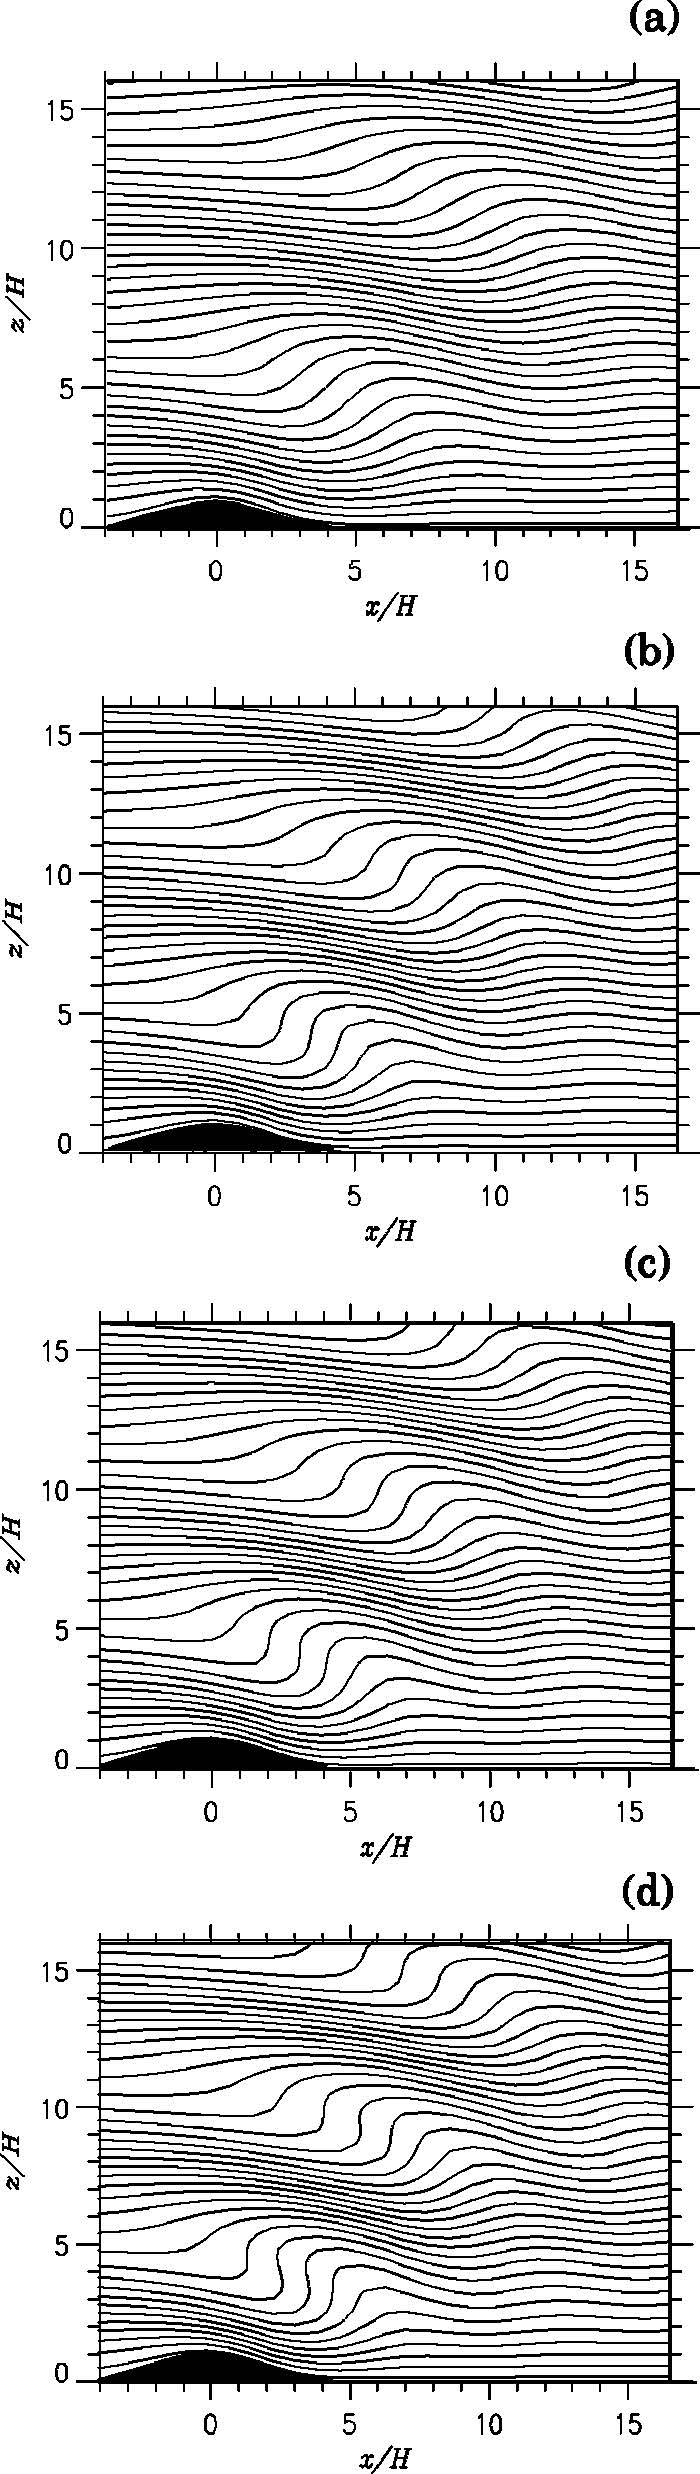
\includegraphics[scale=0.9]{fig/greene_sol}\hspace{1cm}
    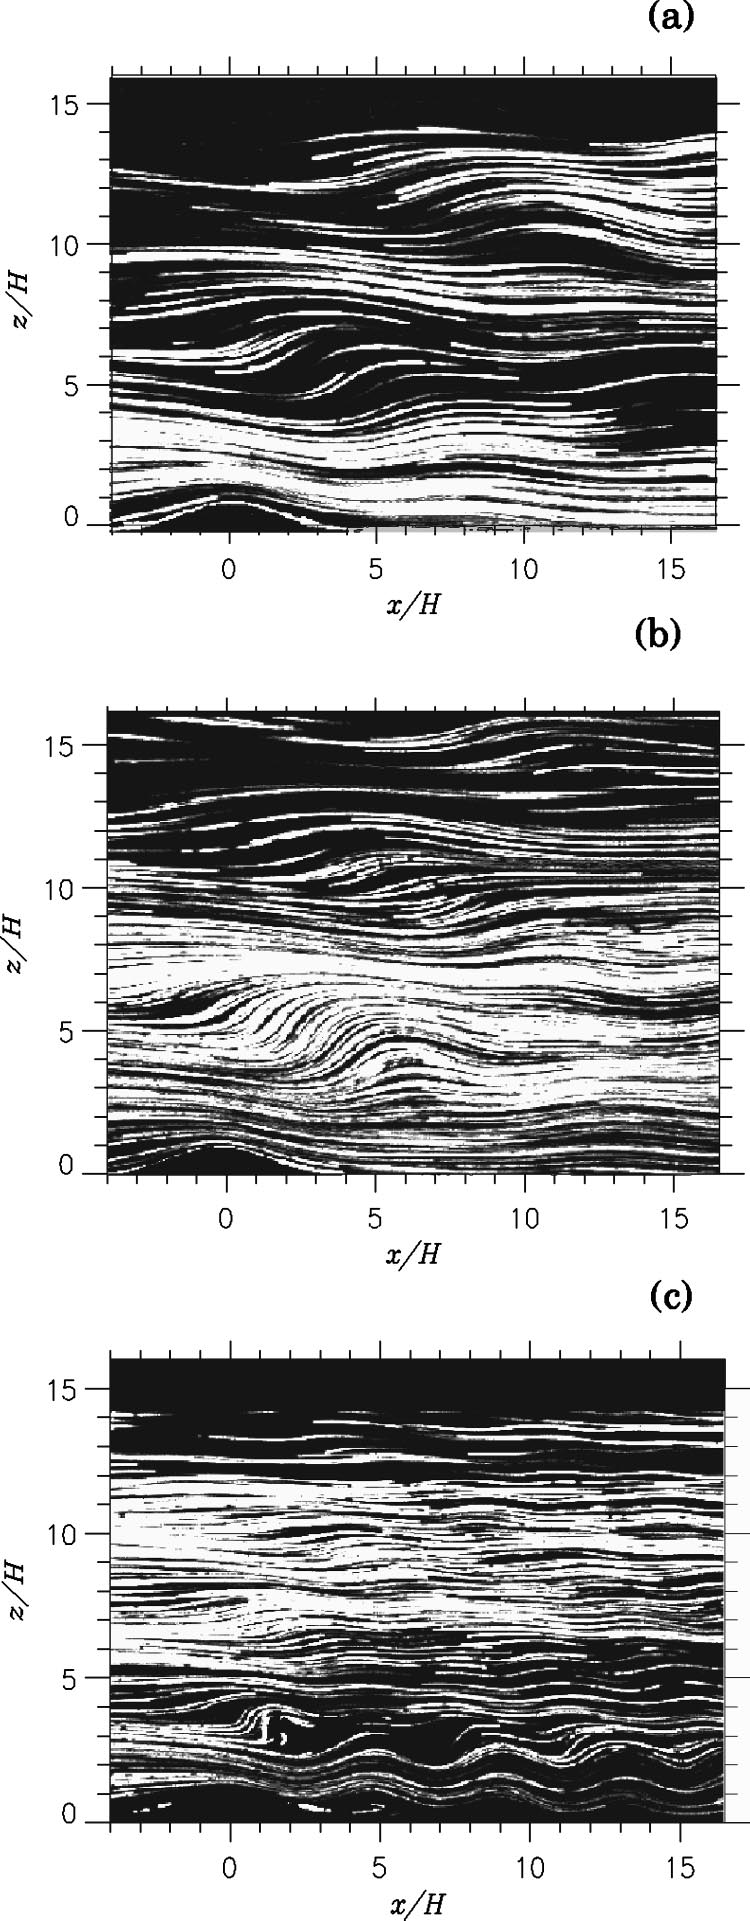
\includegraphics[scale=0.9]{fig/experiement}
    \caption{Original figure captions. Left: FIG. 3. Streamlines over a Gaussian obstacle ($H/L=0.57$) computed from Long’s (1953) two-dimensional inviscid and unbounded model. The flow is from left to right and viewed in the obstacle frame. (a) $\Fr=1.2$, (b) $\Fr=1.0$, (c) $\Fr=0.97$, (d) $\Fr=0.9$. Right: FIG. 4. Pathlines over a two-dimensional Gaussian obstacle ($H/L=0.57$) at $\text{Nt}=150$ and $\text{Re}=150$. (a) $\Fr=1.2$, (b) $\Fr=1.0$, (c) $\Fr=0.6$.}
    \label{fig:from_paper}
\end{figure}

\section{Numerical method}
\subsection{Modification of the numerics}
Since the lee wave problem could be anisotropic in the horizontal and vertical direction, it is beneficial to simulate a non-square domain with different grid sizes in the horizontal and vertical. We have modified the 2D Matlab code to allow for anisotropic domain and discretization. 

\subsection{Target point for the topography}
To represent the topography, we use target points. Each point is tethered to a prescribed target location using a linear stiff spring. The force for each point is
\begin{align}
    \ve F_i = -K(\ve X_i-\ve X_i^\text{target}).
\end{align}
It act on the point to keep is close to the intended location, and it act on the fluid to represent the effects of the boundary on the fluid.

\subsection{Penalty points representing excess mass}\label{sec:pIBM}
We could just evolve \eqref{eq:bouy_eq} in time by solving the linear advection problem. However, in the spirit of pIBM, we represent excess mass using penalty points. They are advected by the fluid velocities and represent the gravitational force of the excess mass by spreading the gravity force onto the fluid. At the beginning time, we seed points in the whole domain, each carrying a value of buoyancy at its location. After 5 CFL time, we interpolate the now advected point into a uniform dense grid in the whole domain. Doing re-gridding often make sure that there are no region in the fluid that have an excess or a lack of buoyancy points. This procedure is familiar to one who uses semi-Lagrangian numerical methods. 

\section{Results}
\subsection{Sinusoidal topography}
We start with the case where the topography is sinusoidal. That is, we have
\begin{align}
    y^\text{target} = H+H\sin(k x^\text{target})
\end{align}
with $H=0.7125$ and $k=0.375$. We seed the domain with linear buoyancy profile with $N=0.084$. We keep the Reynolds number unrealistically small for our preliminary showcase.

We show the time evolution of the solution in Figure \ref{fig:ib2D_23_t4000} and \ref{fig:ib2D_23_t9168}. We see that in middle time (Figure \ref{fig:ib2D_23_t4000}) the lee wave propagated into the domain, with pattern leaning \emph{against} the mean flow. The buoyancy $b$ develops into wave patterns that is stationary in time and resembles the theoretical solution and experiments. As time progresses further, the lee wave reflects from the rigid top and interacts with the existing waves. This changes the spatial pattern of the lee wave by making it lean less into the mean flow. The details of lee wave interacting with its top reflection is a current topic of research (see for example \cite{BakerMashayek_21}).
\begin{figure}
    \centering
    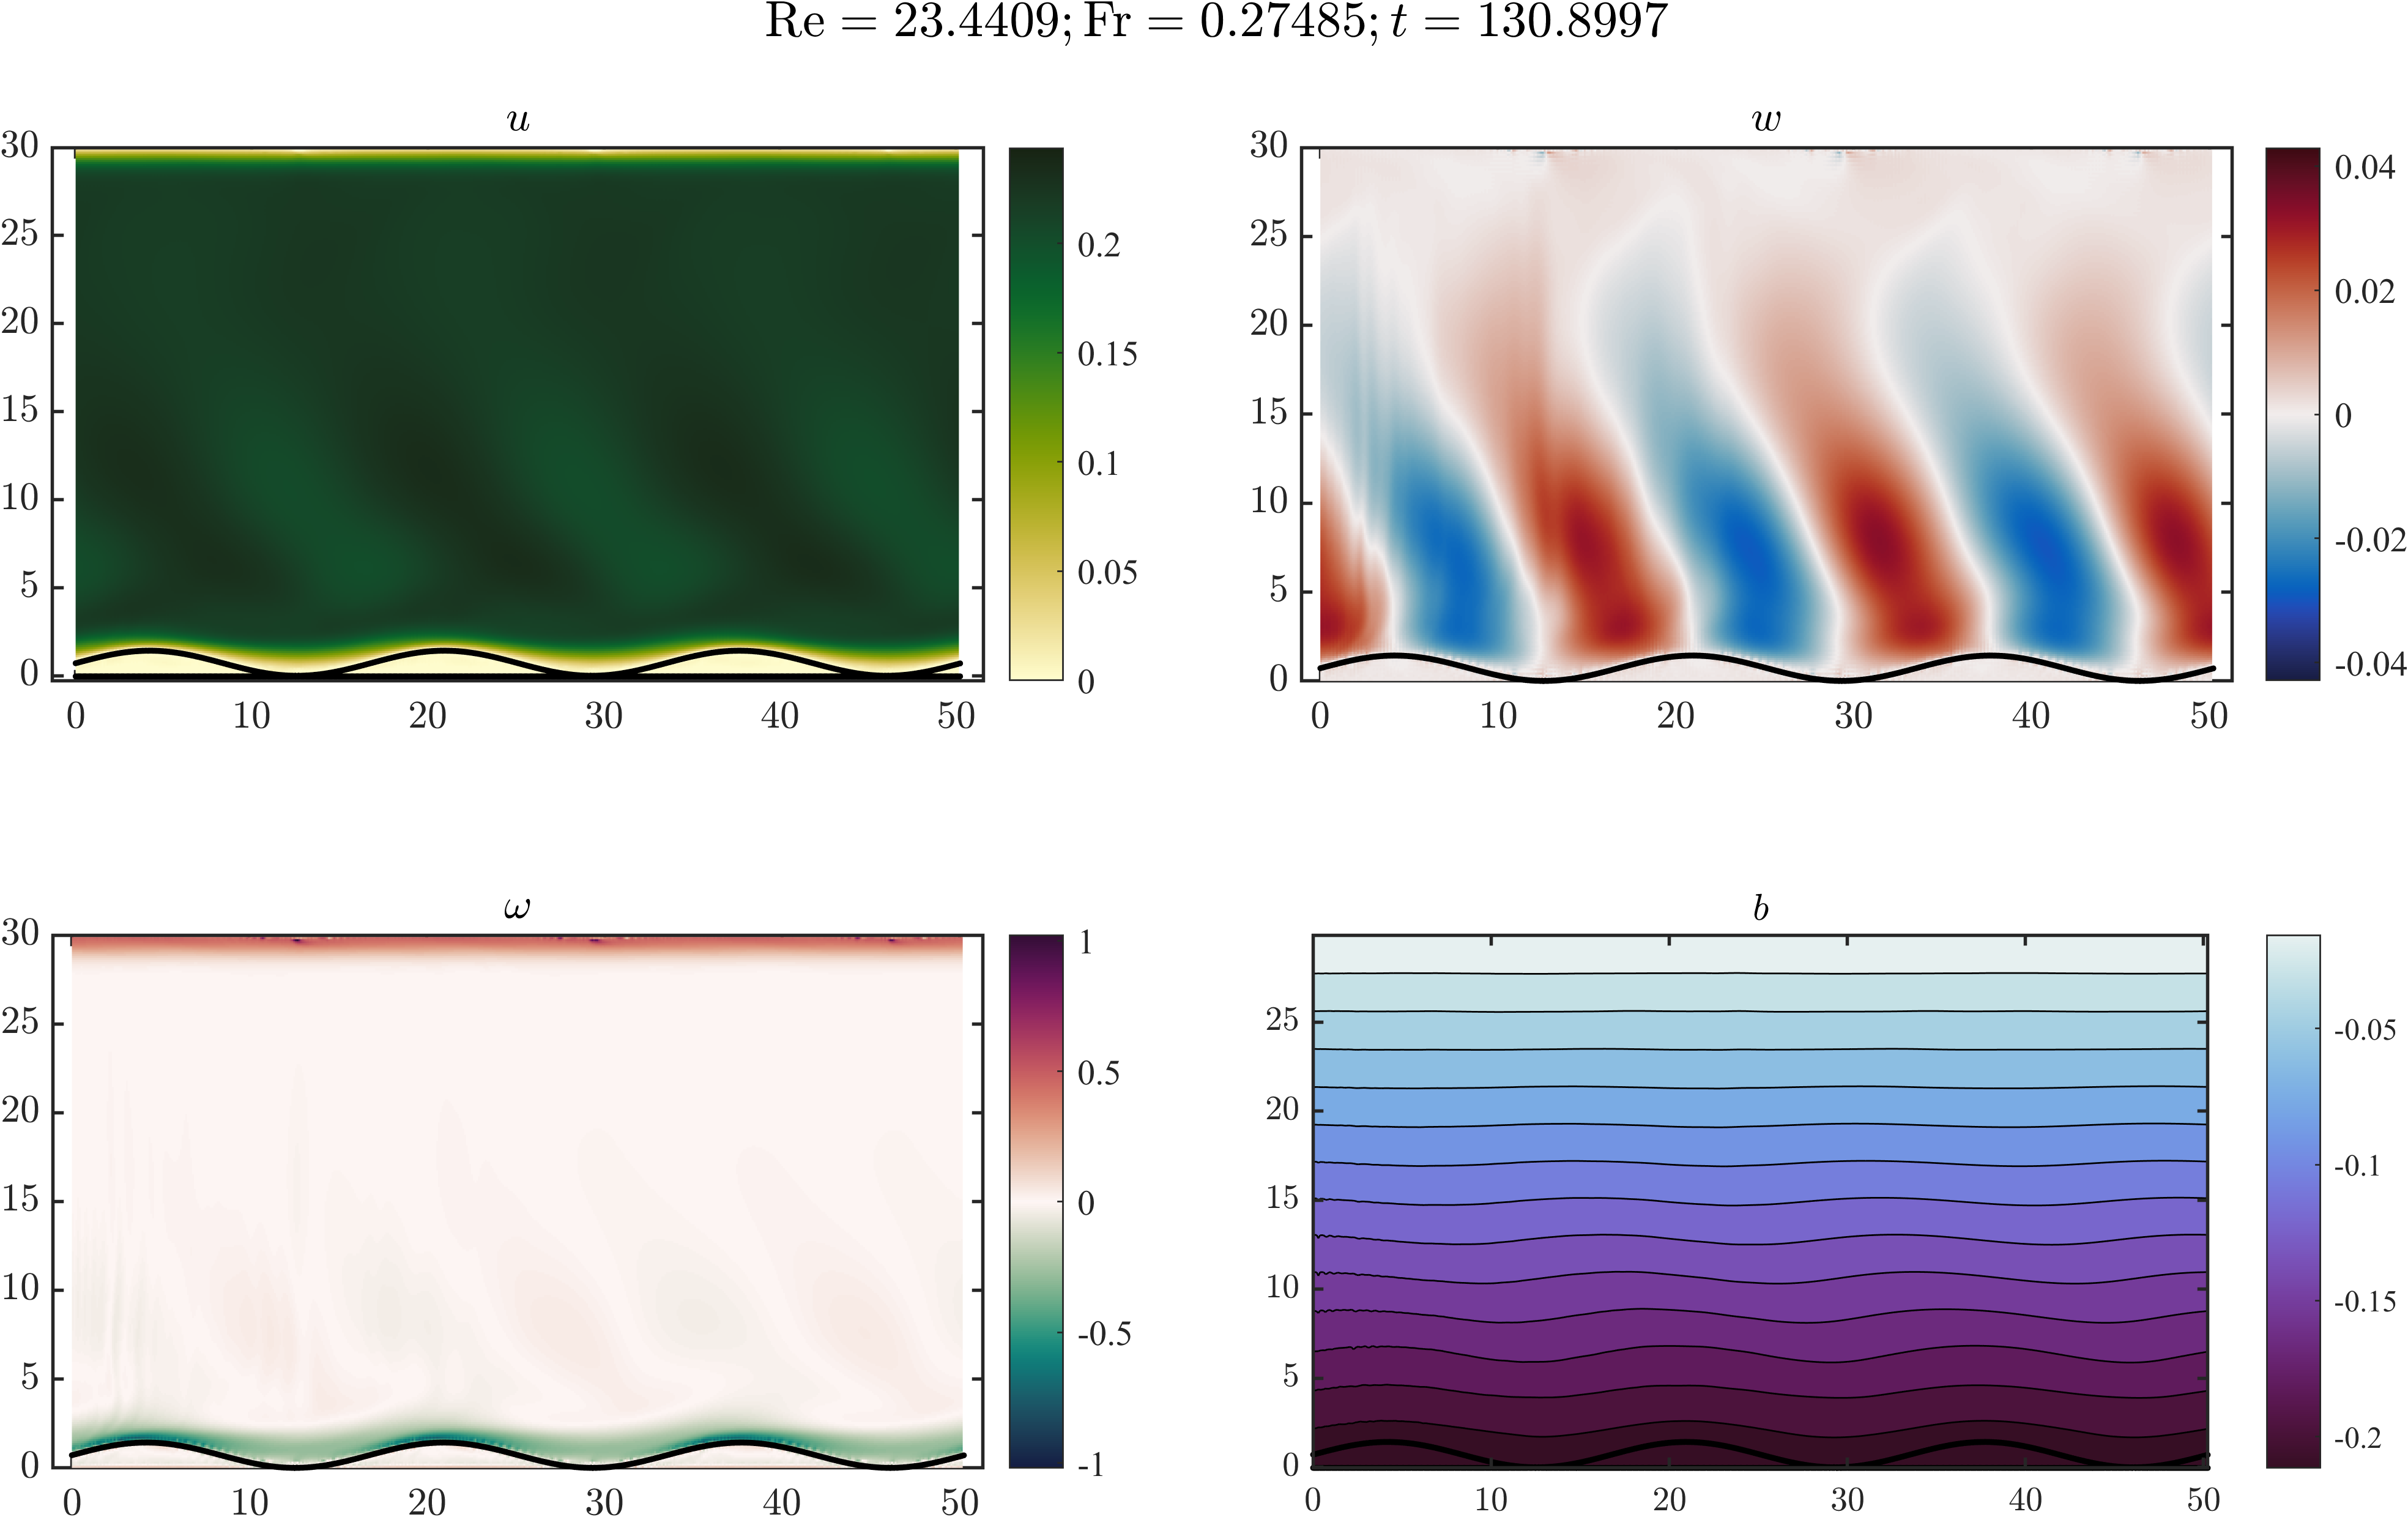
\includegraphics[width=\textwidth]{fig/ib2D_23_t4000}
    \caption{The four panels are: $u$, horizontal velocity; $w$ vertical velocity; $\omega$, vorticity $w_x-u_z$; $b$ buoyancy. }
    \label{fig:ib2D_23_t4000}
\end{figure}
\begin{figure}
    \centering
    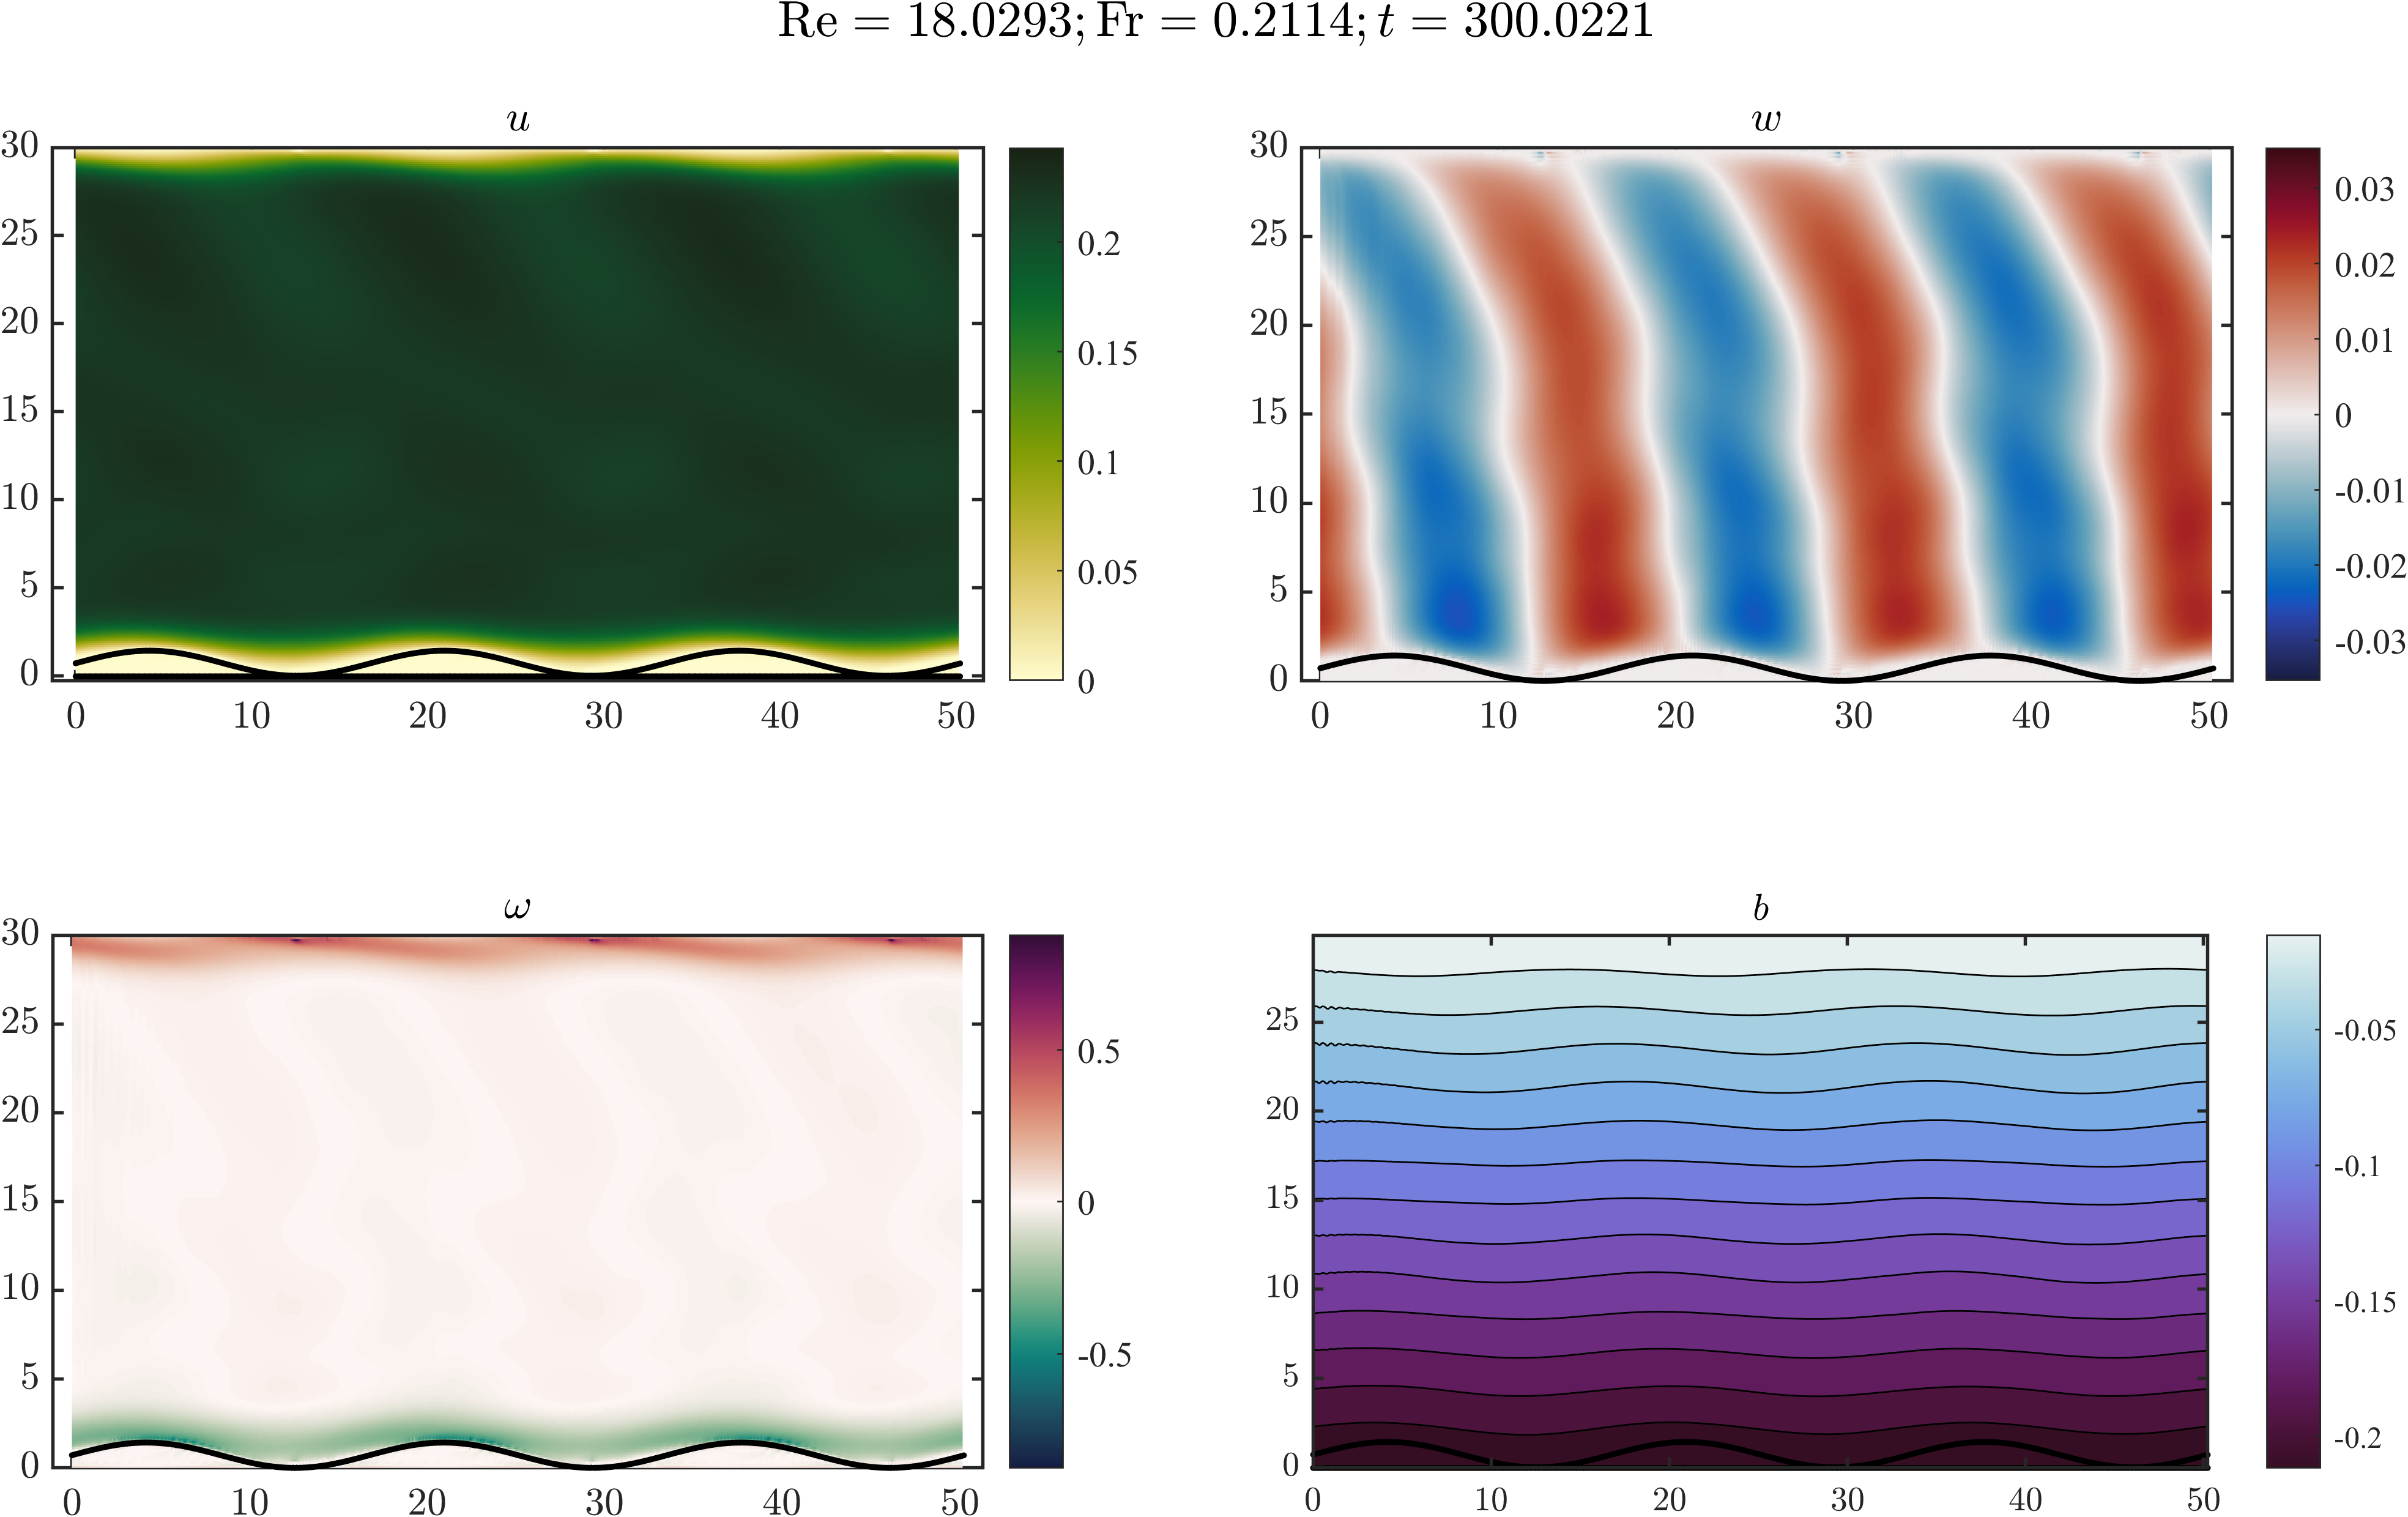
\includegraphics[width=\textwidth]{fig/ib2D_23_t9168}
    \caption{See the caption of Figure \ref{fig:ib2D_23_t4000}.}
    \label{fig:ib2D_23_t9168}
\end{figure}

\subsection{Gaussian topography}
Now we simulate a Gaussian topography, similar to the one in \cite{EiffBonneton_00}. We have
\begin{align}
    y^\text{target} = H\exp\left( -\frac{(x-4L)^2}{2L^2} \right)
\end{align}
with $L = 2$ and $H = 0.57L$. Figure \ref{fig:ib2D_11_t9216} has $N=0.096$ and Figure \ref{fig:ib2D_12_t9216} has $N=0.108$. This give them a slight difference in their Froude number. We see that Gaussian topography produces more complex flow patterns, compared to the sinusoidal case. The perturbation of the density contours are not as large as the ones in Figure \ref{fig:from_paper}, for comparable Froude number. There are several possible reasons. We have too small a Reynolds number, compared to the lab experiment. We have to do this to resolve the boundary layer near the topography. A possible remedy is to use free slip boundary condition for the boundaries. That would require recalculation of the forces. Another possible reason is that the rigid lid is too low. In comparison, the theoretical solution in Figure \ref{fig:from_paper} is for a infinite domain in the vertical. We see from the sinusoidal case that wave reflection affect the wave pattern quickly. It is conceivable that the pressure effect from the top rigid lid suppress the density perturbation. To test this, we could raise the rigid lid, but that would require more computation power and we do not pursue this here.

\begin{figure}
    \centering
    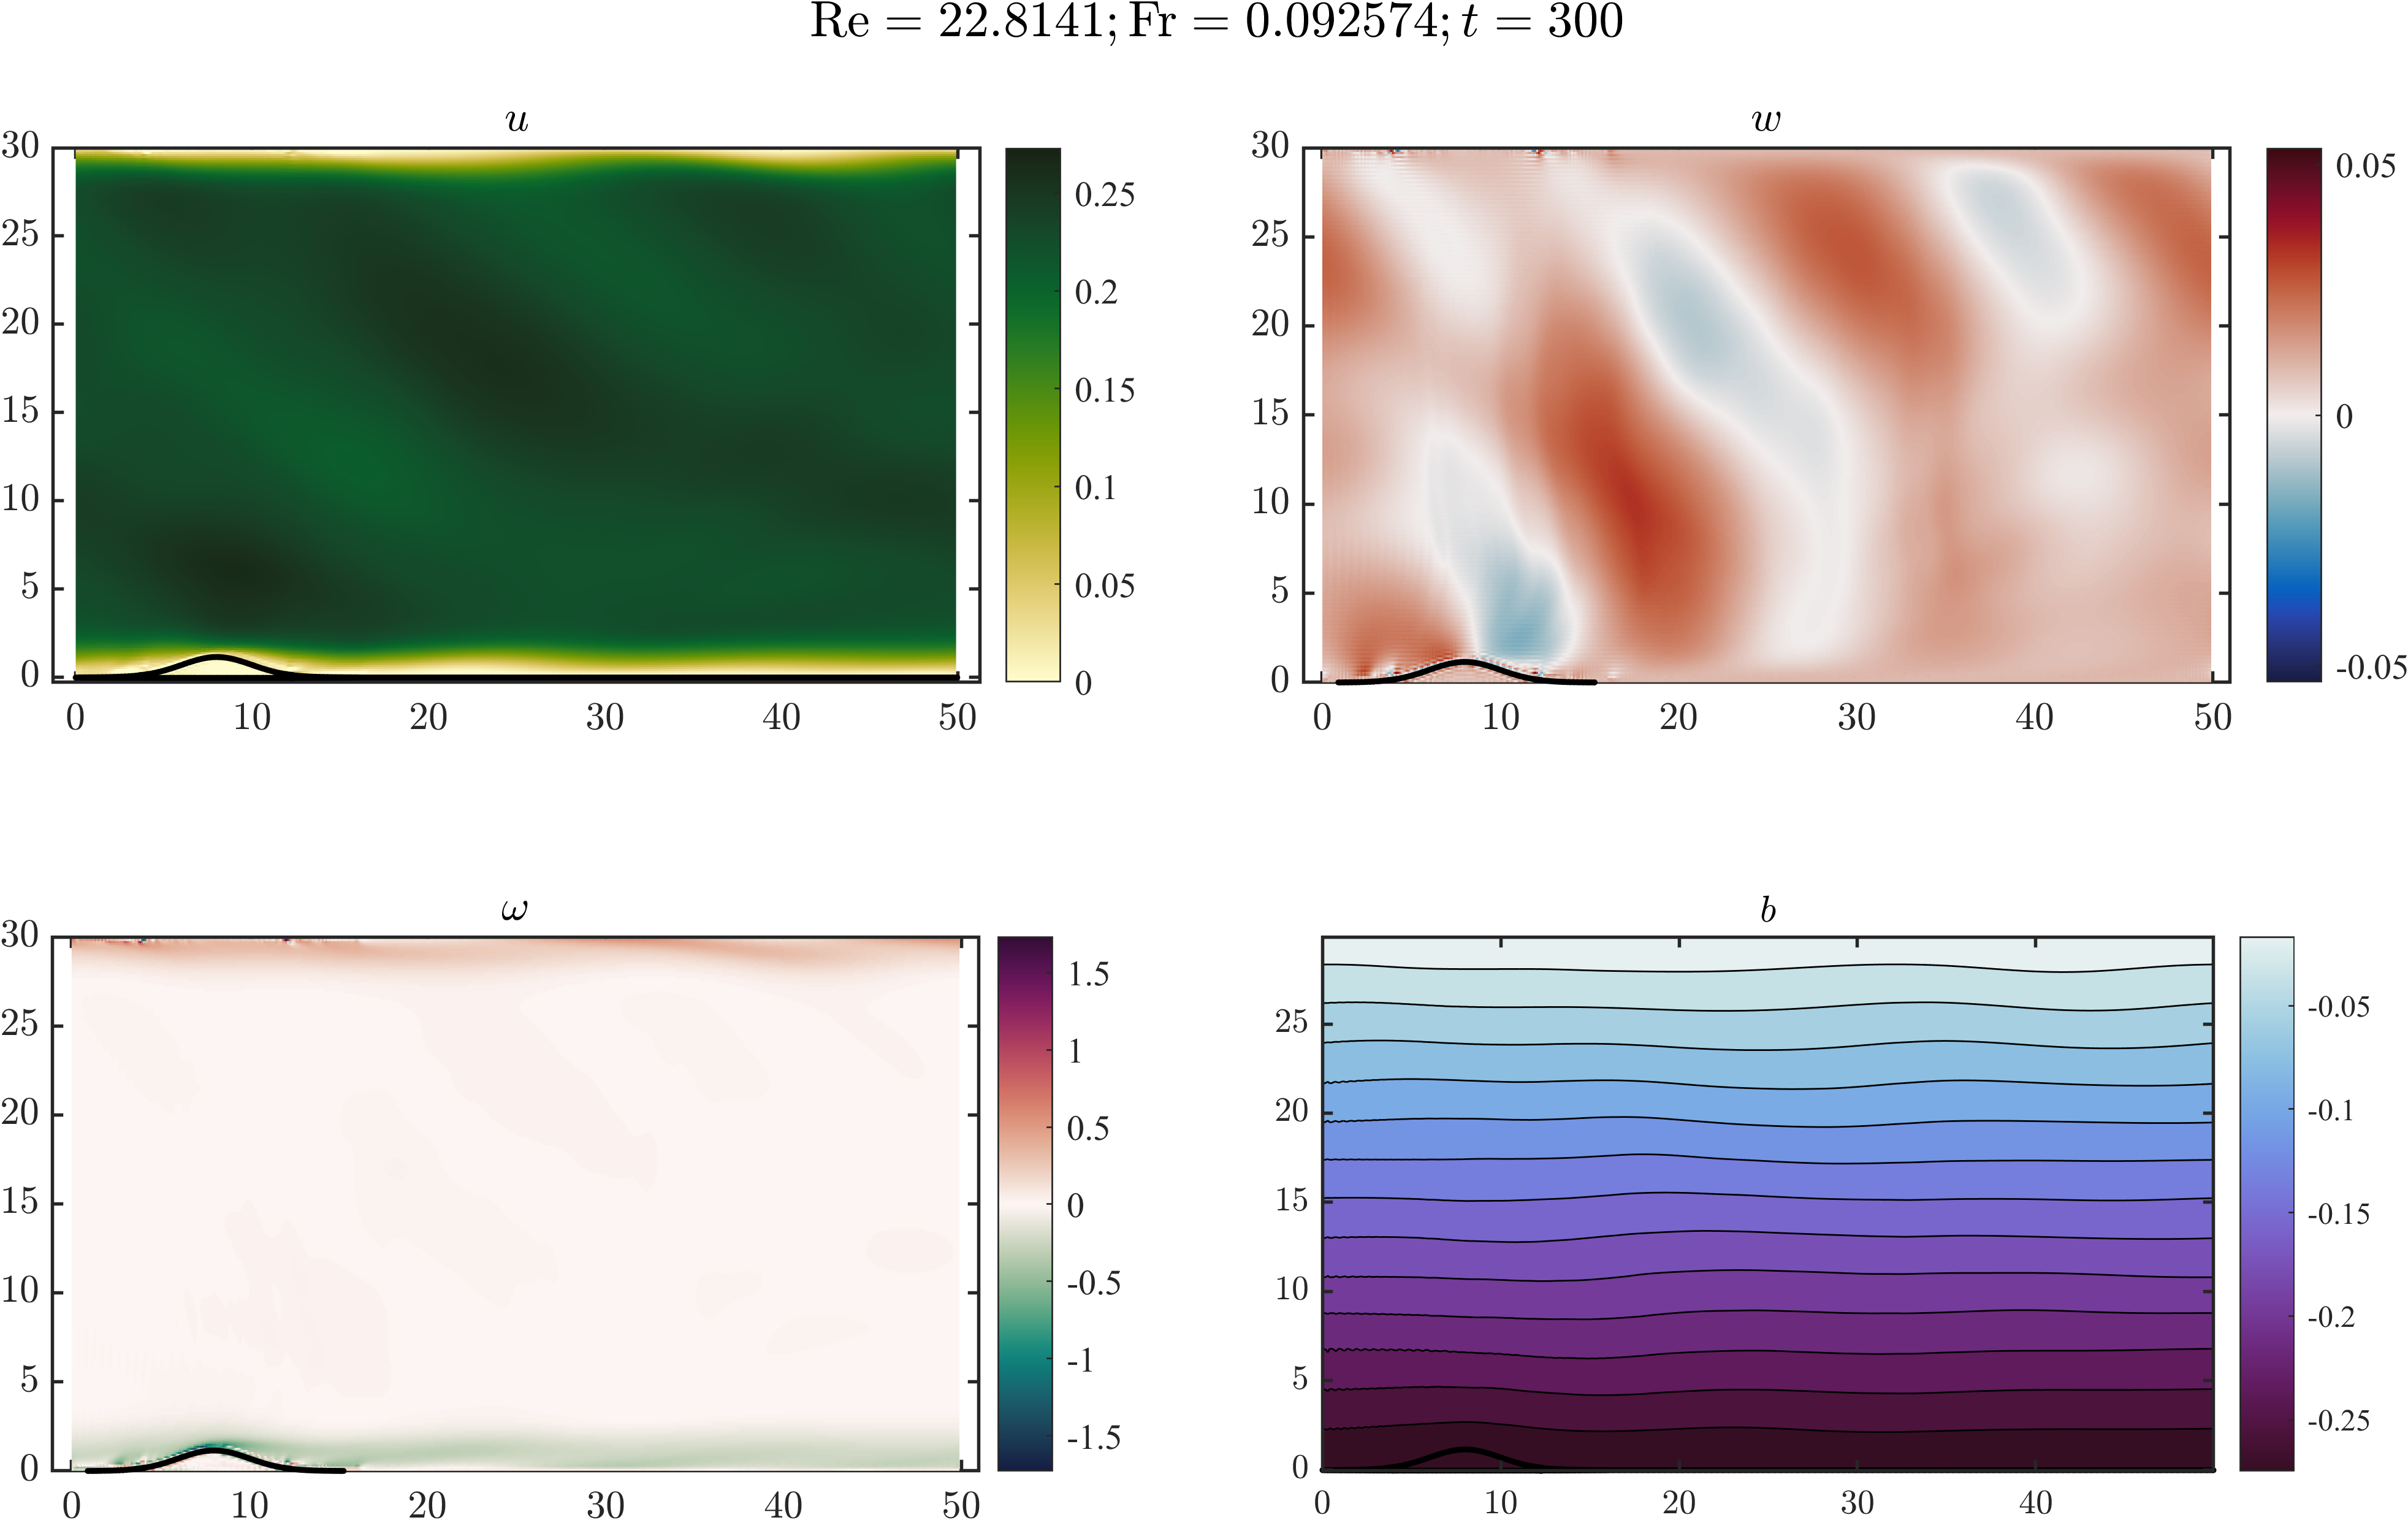
\includegraphics[width=\textwidth]{fig/ib2D_11_t9216}
    \caption{See the caption of Figure \ref{fig:ib2D_23_t4000}.}
    \label{fig:ib2D_11_t9216}
\end{figure}
\begin{figure}
    \centering
    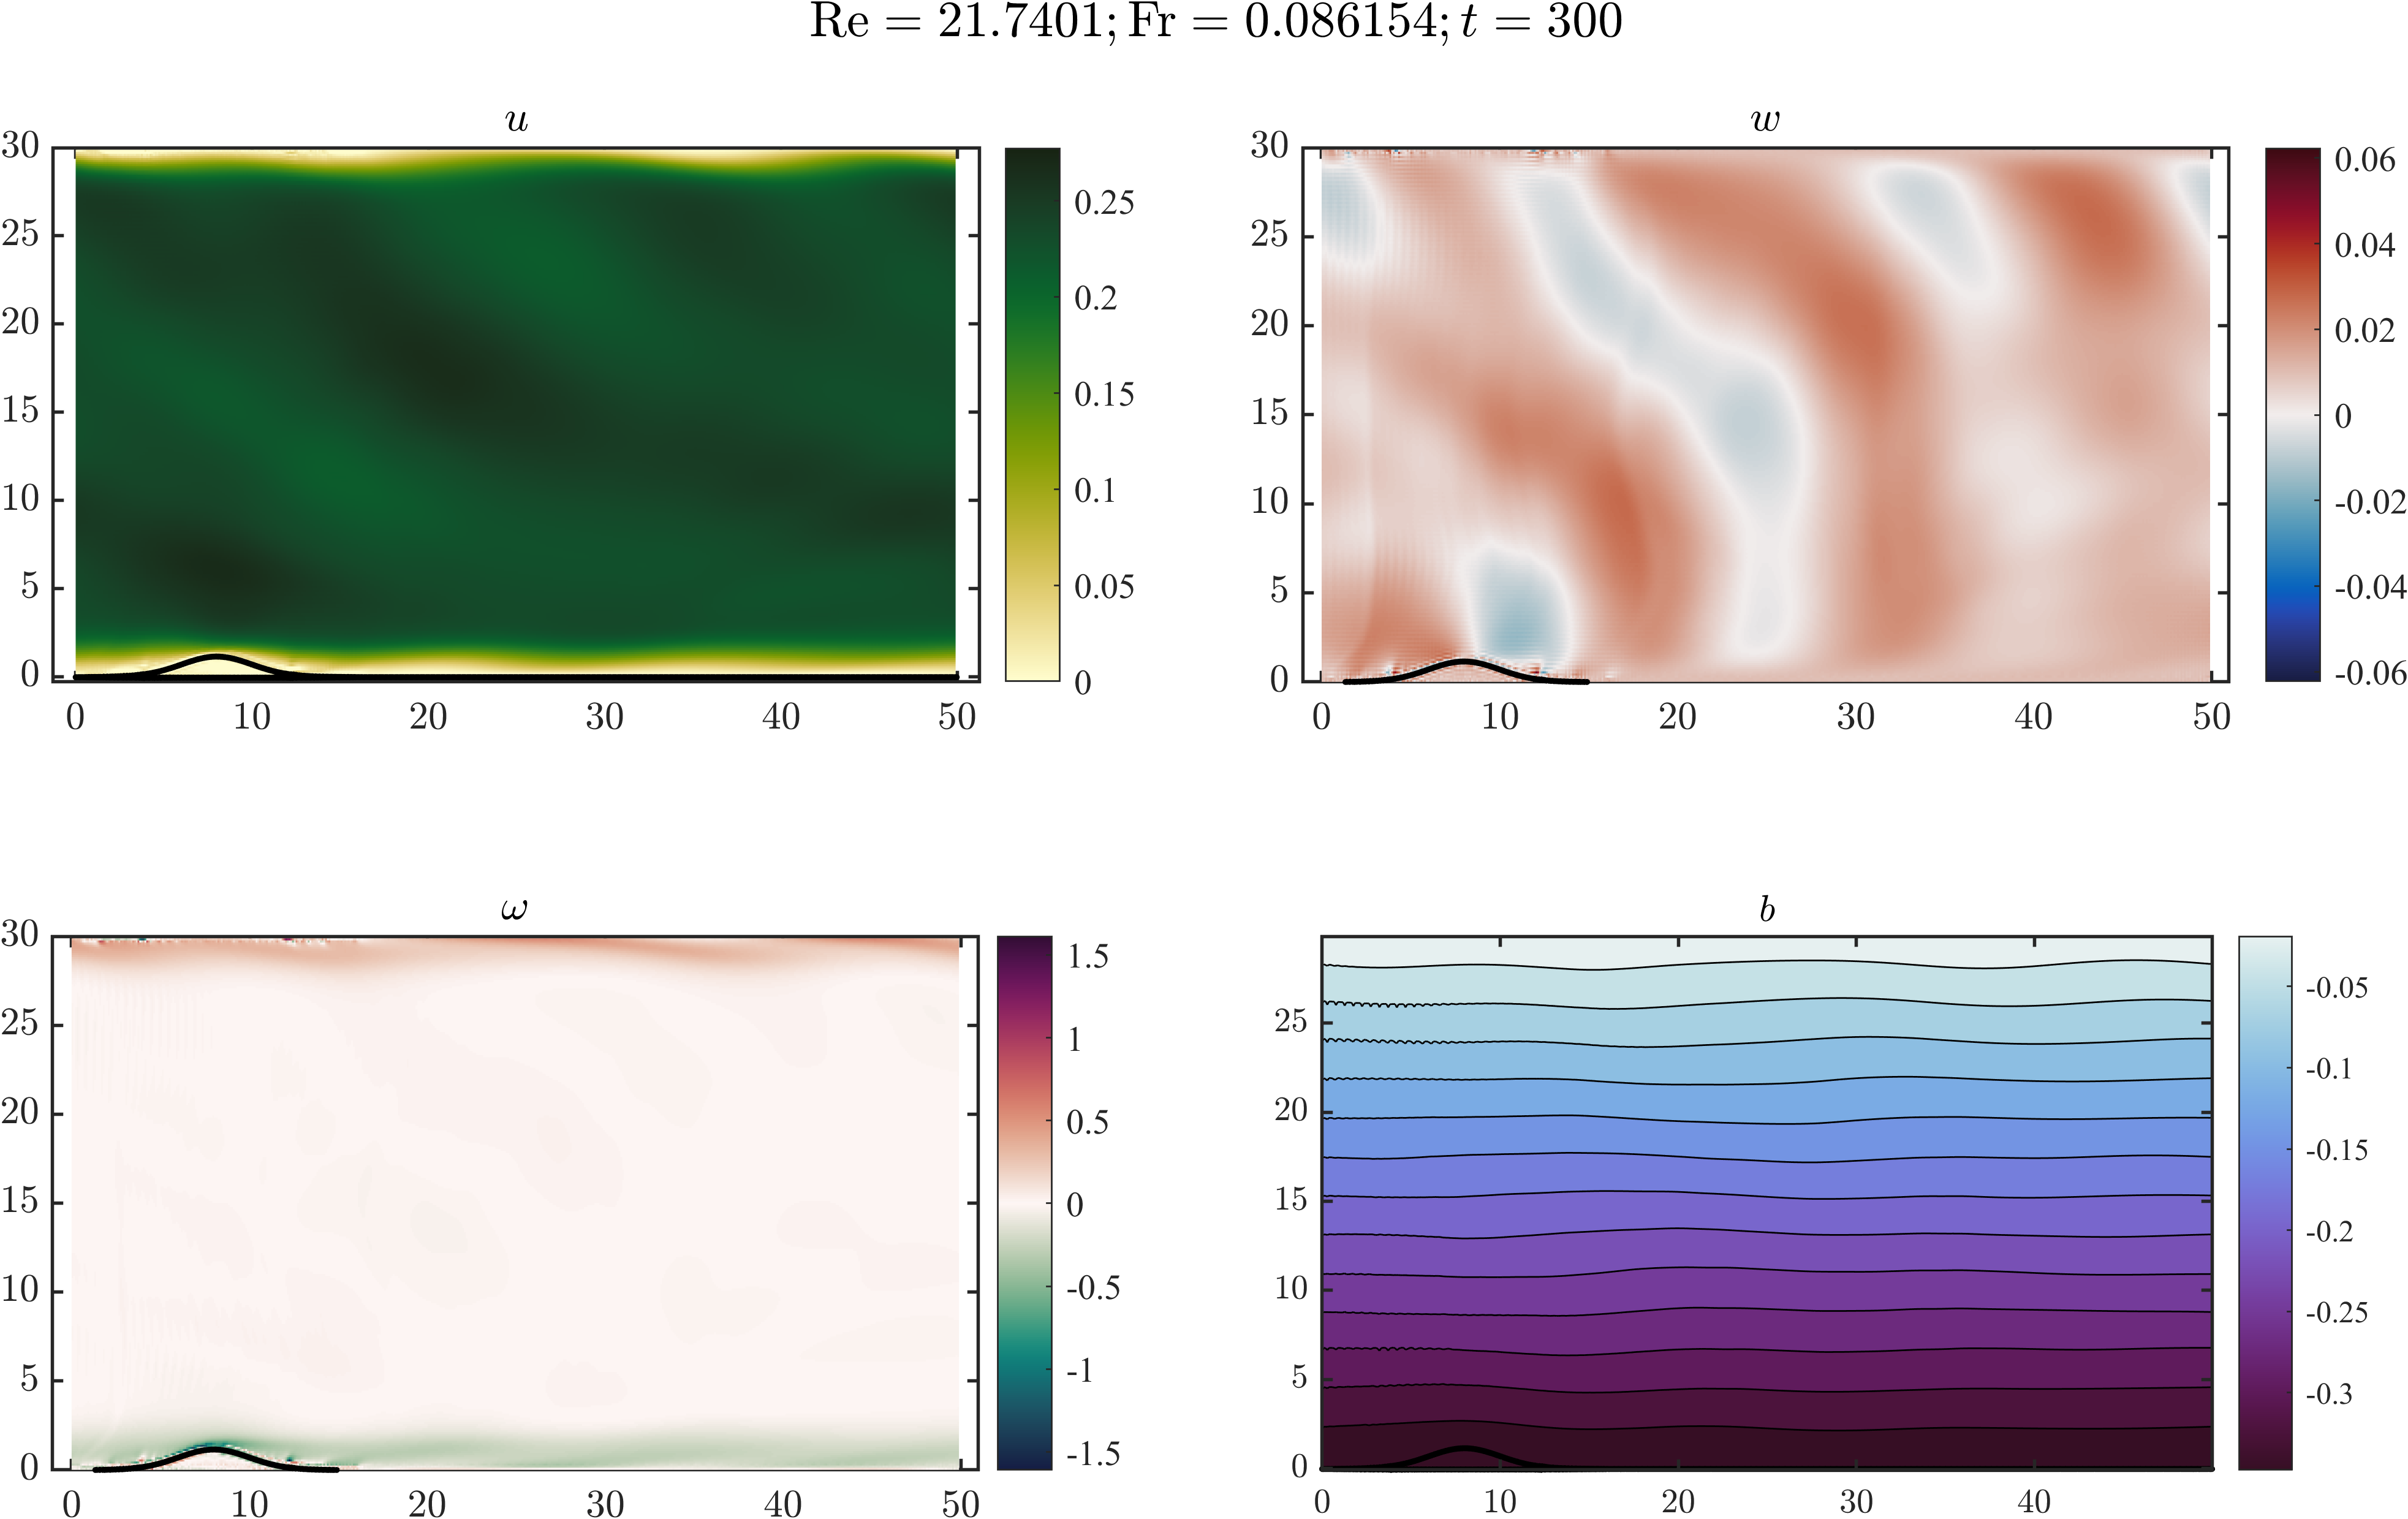
\includegraphics[width=\textwidth]{fig/ib2D_12_t9216}
    \caption{See the caption of Figure \ref{fig:ib2D_23_t4000}.}
    \label{fig:ib2D_12_t9216}
\end{figure}

\section{Conclusions and outlooks}
From a few example simulations, we have shown that pIBM is a viable method to simulate lee waves past a topography. Compared to traditional method that modify the grid near the topography (for example, \cite{AdcroftEtAl_97}), IBM formalism allows for straightforward treatment of complex topographies. However, it is right now unclear to us how the timestep requirement of pIBM method compares to traditional method. The simulation in this note use timestep $O(10)$ times smaller than the CFL requirement because the target point spring is rather stiff. 

An avenue to explore is the separate advection of the density points using a larger timestep. Semi-Lagrangian methods has the advantage that the method is stable for larger timestep, even allowing one to break the CFL requirement \parencite{SpiegelmanKatz_06}. The simulations in this note use the same small timestep to advect the density point. But it might be better for computational cost to use a larger timestep, larger than the one used for the fluid solver.

\appendix
\section{Code availability}
The code used in this report is available at \url{https://github.com/Empyreal092/lee_wave_IBM}. 


\vfill
\printbibliography

\end{document}
